\documentclass{beamer}
\usetheme{Berlin}

\title{Fast Decision Procedures Based on Congruence Closure}
\author{Sven Keidel}
\date{\today}

\usepackage[utf8]{inputenc}

\usepackage{fancyvrb}
\usepackage[cache]{minted}
\newmintedfile{haskell}{
  fontsize=\footnotesize
}

\usepackage{tikz}
\usetikzlibrary{arrows,positioning,decorations.pathmorphing}
\tikzstyle{vertex}=[circle,draw,minimum size=0.7cm]
\tikzstyle{edge}=[->, >=latex,draw]

\begin{document}

\maketitle

\section{Introduction}

\begin{frame}
  \frametitle{Objective and Motivation}

  \begin{itemize}
    \item Decision procedure for the quantifier-free theory of equality with
      uninterpreted function symbols.
      \begin{itemize}
        \item $f(a) = a \rightarrow f(f(a,b),b) = a$
        \item $0 = 1$
      \end{itemize}

    \item Determines the satisfiability of a conjunction of
      literals of length $n$ in $O(n \log n)$.

    \item Can be extended to theories with interpreted function symbols like the
      theory of lists.
  \end{itemize}

\end{frame}


\subsection{Definitions}

\begin{frame}
  \frametitle{Definition of a Term Graph}

  \begin{Definition}[Term Graph]
    \begin{itemize}
      \item Let $G = (V,E)$ be a directed graph.
      \item Let $\lambda(v)$ be the label of a vertex $v$.
      \item Let $\sigma(v)$ be the outdegree of a vertex $v$.
      \item Leaving edges are ordered. Let $v[i]$ denote the $i$th successor of
        $v$, where $1 \leq i \leq \sigma(v)$.
      \item Multiple edges are allowed, so it is possible that $v[i] = v[j]$ for
        $i \neq j$.
    \end{itemize}
  \end{Definition}

\end{frame}

\begin{frame}
  \frametitle{Example of a Term Graph}

  \begin{columns}
    \begin{column}{0.5\textwidth}
      Term graph of the terms $f(f(a,b),b)$, $f(a,b)$, $a$ and $b$.
    \end{column}
    \begin{column}{0.5\textwidth}
      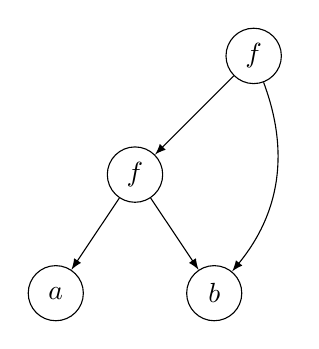
\begin{tikzpicture}
        \node [vertex] (v1) {$f$};
        \node [vertex,below left=of v1] (v2) {$f$};
        \node [vertex,below left=of v2,xshift=0.50cm] (v3) {$a$};
        \node [vertex,below right=of v2,xshift=-0.50cm] (v4) {$b$};

        \path [edge] (v1) -- (v2);
        \path [edge] (v1) edge [bend left] (v4);
        \path [edge] (v2) -- (v3);
        \path [edge] (v2) -- (v4);
      \end{tikzpicture}
    \end{column}
  \end{columns}
\end{frame}

\begin{frame}
  \frametitle{Definition of Congruence}

  \begin{Definition}[Congruence]
    \begin{itemize}
      \item Let $R \subset V \times V$ be a relation.
      \item Two vertices $u$ and $v$ are \textit{congruent under $R$} iff
        \begin{itemize}
          \item $\lambda(u) = \lambda(v)$,
          \item $\sigma(u) = \sigma(v)$ and
          \item forall $i$ s.t. $1 \leq i \leq \sigma(u)$, $u[i] = v[i]$.
        \end{itemize}
      \item $R$ is \textit{closed under congruences} if, forall vertices $u$ and
        $v$ s.t. $u$ and $v$ are \textit{congruent under $R$}, $(u,v) \in R$.
    \end{itemize}
  \end{Definition}

\end{frame}


\begin{frame}
  \frametitle{The Congruence Closure of $R$}

  \begin{Lemma}[Congruence Closure]
    There is a unique minimal extension $R'$ of $R$ s.t. $R'$ is an equivalence
    relation and $R'$ is closed under congruences; $R'$ is the
    \textit{congruence closure} of $R$.
  \end{Lemma}
\end{frame}

\section{Implementation}

\begin{frame}[fragile]
  \frametitle{$\mathbf{congruent}(u, v)$}

  \begin{columns}[T]
    \begin{column}{0.5\textwidth}
      \haskellfile
        [ firstline=101
        , lastline=106
        ]
        {../src/Logic/CongruenceClosure.hs}
    \end{column}
    \begin{column}{0.5\textwidth}
      \begin{enumerate}
        \item if $\sigma(u) \neq \sigma(v)$, then return $\mathbf{false}$
        \item for $1 \leq i \leq \sigma(u)$, if $\mathbf{find}(u[0]) \neq \mathbf{find}(v[t])$,
          then return $\mathbf{false}$
        \item return $\mathbf{true}$
      \end{enumerate}
    \end{column}
  \end{columns}
\end{frame}

\begin{frame}[fragile]
  \frametitle{$\mathbf{merge}(u,v)$}
  \framesubtitle{Produces the Congruence Closure of $R \cup \{(u,v)\}$}

  \begin{columns}[T]
    \begin{column}{0.5\textwidth}
      \haskellfile
        [ firstline=75
        , lastline=88
        ]
        {../src/Logic/CongruenceClosure.hs}
    \end{column}
    \begin{column}{0.5\textwidth}
      \begin{enumerate}
        \footnotesize
        \only<1>{
          \item If $\mathbf{find}(u) = \mathbf{find}(v)$, then return.
          \item Let $P_u$ be the set of all predecessors of all vertices equivalent
            to $u$, and $P_v$ the set of all predecessors of all vertices
            eqivalent to $v$.
          \item Call $\mathbf{union}(u, v)$.
        }
        \setcounter{enumi}{3}
        \only<2>{
          \item For each pair $(x, y)$ such that $x \in P_v$, and $y \in P_o$, If
            $\mathbf{find}(x) = \mathbf{find}(y)$ but $\mathbf{congruent}(x, y) =
            \mathbf{true}$,
            then $\mathbf{merge}(x, y)$.
        }
      \end{enumerate}
      \begin{itemize}
        \only<3>{
          \item Runtime complexity of $\mathbf{merge}(x,y)$ is $O(m^2)$ where
            $m$ is the number of edges of the Graph.
          \item With a more sophisticated version of step 4, the runtime
            complexity can be reduced to $O(m \log m)$.
        }
      \end{itemize}
    \end{column}
  \end{columns}
\end{frame}

\section{Proofs}

\end{document}
